\begin{figure}[t]
    \centering
	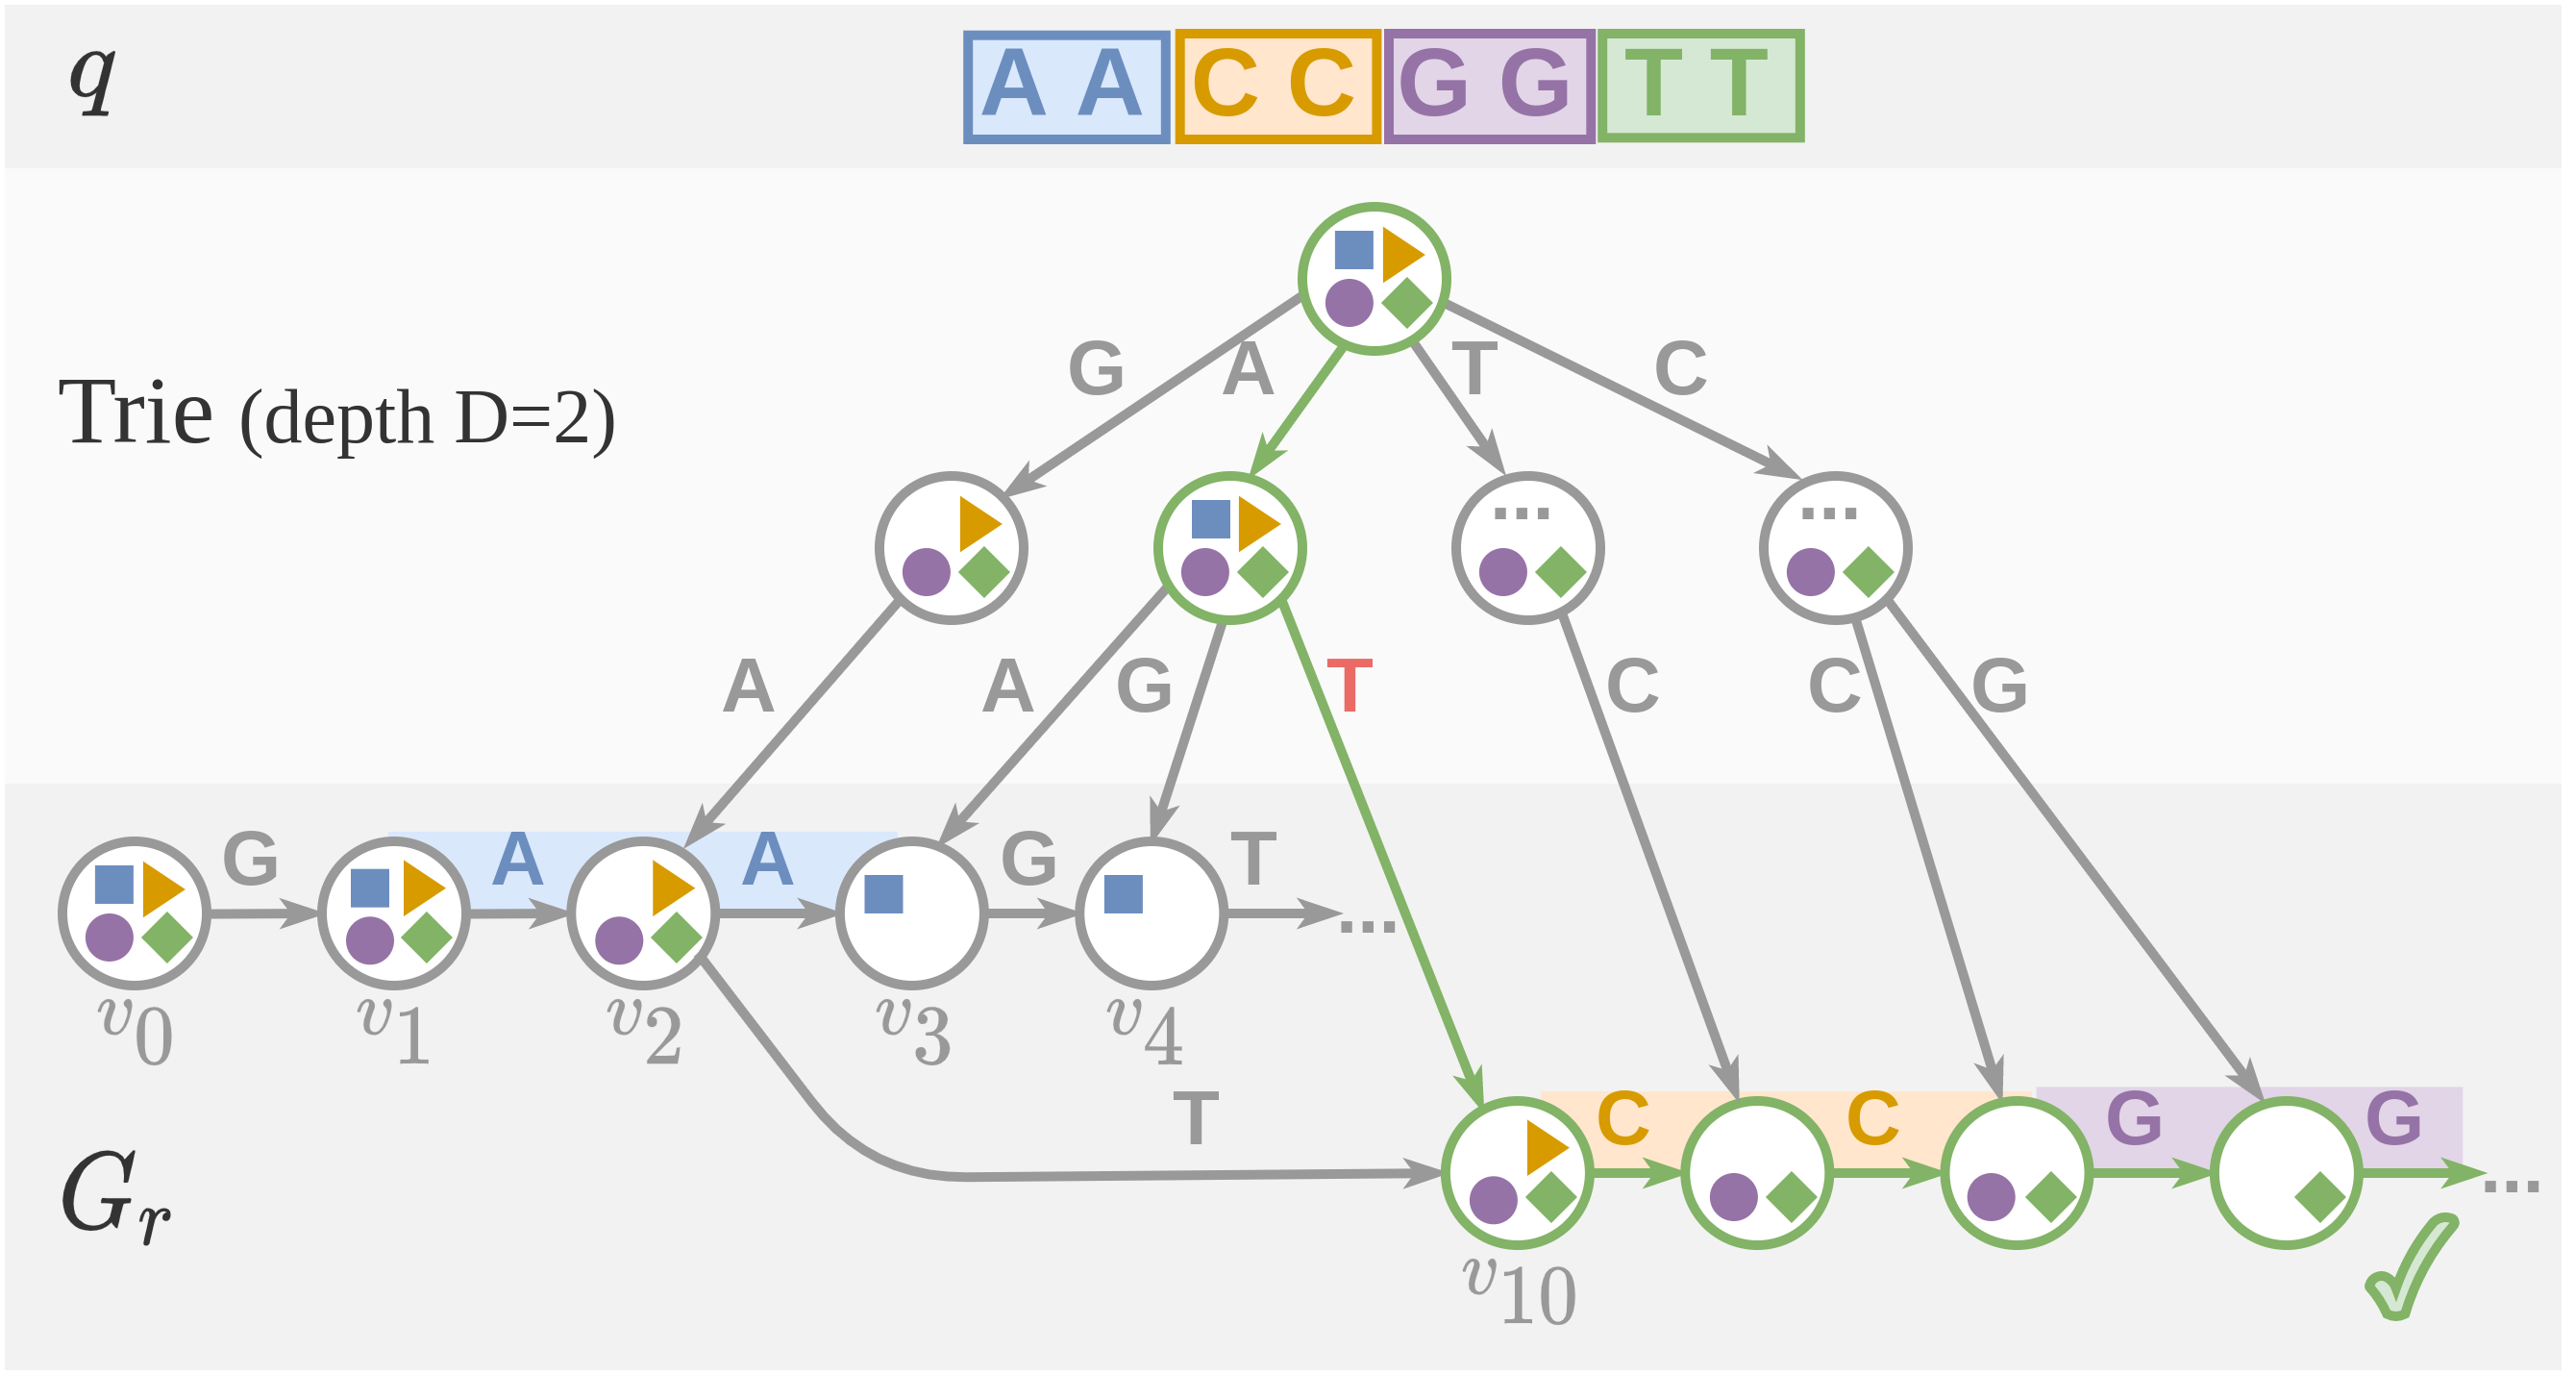
\includegraphics[width=0.6\linewidth]{figures/crumbs-trie.png}
	\caption{Reference graph from \cref{fig:overview}, extended by a trie of
	depth $D=2$. For simplicity, the reverse-complement reference graph and
	parts marked by ``\dots'' are omitted.}
	\label{fig:trie}
\end{figure}

\subsection{On a trie index} \label{SEEDsec:trie}
%
Considering all nodes $v \in \RGV$ as possible starting points for the alignment
means that the \A~algorithm would explore all states of the form $\st{v}{0}$,
which immediately induces a high overhead of $\lvert \RGV \rvert$.
%
In line with the previous section, we avoid this overhead by complementing the
reference graph with a trie index to produce a new graph $\TG = (\TGV, \TGE)$,
where $\TGV$ is the union of the reference graph nodes $\RGV$ and the new trie
vertices, and $\TGE$ is the union of $\RGE$, the trie edges, and edges
connecting the trie leafs with reference nodes. Note that constructing this trie
index is a one-time pre-processing step that can be reused for multiple queries.

Since we want to also support aligning reverse-complement reads by starting from
the trie \trieroot{}, we build the trie not only from the original reference
graph and also from its reverse-complement.

\paragraph{Intuition}
%
\cref{SEEDfig:trie} extends the reference graph $\RG$ from \cref{SEEDfig:overview} with
a trie. Here, any path in the reference graph uniquely corresponds to a path
starting from the trie \trieroot{} (the top-most node in \cref{SEEDfig:trie}). Thus,
in order to find an optimal alignment, it suffices to consider paths starting
from the trie \trieroot{}, by using state $\st{\trieroot}{0}$ as the only source
for the \A~algorithm.
%
Note that if the reference graph branches frequently, the number of paths with
length $D$ may rise exponentially, leading to an exponential number of trie
leaves. To counteract this exponential growth, we can select $D$ logarithmically
small, as $\log_4N$.

Importantly, our placement of crumbs~(\cref{SEEDsec:definition}) generalizes
directly to reference graphs extended with a trie (see also
\cref{SEEDfig:trie}).

% This leads to the effect that the crumbs in a trie node correspond to the
% union of the crumbs of its descendents (with the exception when crumbs are
% skipped for propagating to the trie \cref{SEEDpara}).

\paragraph{Reusing the trie to find seed matches}
%
As a second usage of the trie, we can also exploit it to efficiently locate all
matches $M(s)$ of a given seed $s$.
%
In order to find all nodes where a seed match begins, we align (without errors)
$\bar{s}$, the reverse-complement of $s$. To this end, we follow all paths
spelling $\bar{s}$ starting from the $\trieroot$---the final nodes of these
paths then correspond to nodes in $M(s)$. We ensure that the seed length $|s|$
is not shorter than the trie depth $D$, so that matching all letters in
$\bar{s}$ ensures that we eventually transition from a trie leaf to the
reference graph.

% Analogously, our computation of crumbs (\cref{SEEDsec:algo} and \cref{SEEDalg:crumbs})
% generalizes directly to reference graphs extended by a trie.
% %
% However, assuming that we select the depth of the trie to be the same as the
% length of each seed ($D=k$) allows us to speed up the computation by only
% starting the search for matches of a seed in~$\varepsilon$.
% %
% Specifically, in \cref{SEEDalg:crumbs}, we can replace \cref{SEEDlin:match-init} by $T
% \gets \{\varepsilon\}$. This is because
% \crefrange{lin:match-forward-start}{lin:match-forward-end} will locate all nodes
% in the original reference graph which can be the end point of a seed match.
% Then, \crefrange{lin:match-backward-start}{lin:match-backward-end} will
% backtrack both in the reference graph as well as in the trie, thus ensuring that
% $M(s)$ is computed correctly.

\paragraph{Optimization: skip crumbs on the trie} \label{SEEDpar:skip_crumbs}
%
Generally, we aim to place as few crumbs as possible, in order to both reduce
precomputation time and avoid misleading the \A~algorithm by unnecessary crumbs.
In the following, we introduce an optimization to avoid placing crumbs on trie
nodes that are ``too close'' to the match of their corresponding seed so they
cannot lead to an optimal alignment.

Specifically, when traversing the reference graph backwards to place crumbs for
a match of seed $s$ starting at node $w$, we may ``climb'' from a reference
graph node $u$ to a trie node $u'$ backwards through an edge that otherwise
leads from the trie to the reference.
%
Assuming $s$ starts at position $i$ in the read, we have already established
that we can only consider nodes $u$ that can reach $w$ with less than
$i+\maxdel$ edges (see \cref{SEEDsec:definition}).
%
Here, we observe that it is sufficient to only climb into the trie from nodes
$u$ that can reach $w$ using more than~$i-\maxins-D$ edges, for
\begin{align}
	\maxins := \left\lceil \frac{\lvert q \rvert \cdot \cmatch + |\seeds| \cdot \delta_{\mli{min}}}{\cins} \right\rceil.
\end{align}
%
We define $\maxins$ analogously to $\maxdel$ to ensure that $\maxins$ insertions
will induce a cost that is always higher than $h\st{u}{i}$. We note that we can
only avoid climbing into the trie if all paths from $u$ to $w$ are too short, in
particular the longest one.

The following \cref{SEEDlem:trie-optimization} shows that this optimization
preserves optimality.

\begin{lem}[Admissibility when skipping crumbs]
	\label{SEEDlem:trie-optimization}
	The \sh remains admissible when crumbs are skipped in the trie.
\end{lem}
\begin{proof}
	Consider a reference graph with a match of seed $s$ starting in node $w$.
	Now, consider a node $v$ that cannot reach $w$ using more than $i-D-\maxins$
	edges.
	%
	We can then show that a trie node $v'$ with a path to $v$ does not require a
	crumb for the match of $s$ in node $w$.

	Specifically, any path from $\trieroot$ through nodes $v'$ and $v$ to node
	$w$ has total length greater or equal $i-\maxins$. Thus, matching $s$ at $w$
	requires at least $\maxins$ insertions. Hence, the cost of such a path is at
	least $\maxins \cdot \cins = |q| \cdot \cmatch + n \cdot
	\delta_{\mli{min}}$. Observing that this is an upper bound for $h\st{v}{i}$
	concludes the proof.
\end{proof}

In order to efficiently identify all nodes $u$ that can reach $w$ by using more
than $i-D-\maxins$ edges (among all nodes at a backward-distance at most
$i+\maxdel$ from $w$), we use topological sorting: considering only nodes at a
backward-distance at most $i+\maxdel$ from $w$, the length of a longest path
from a node $v$ to $w$ is (i)~$\infty$ if $v$ lies on a cycle and
(ii)~computable from nodes closer to $w$ otherwise.
